\documentclass[border=10pt,tikz]{standalone}
\usepackage{tikz}
\usetikzlibrary{positioning,arrows.meta}
\begin{document}
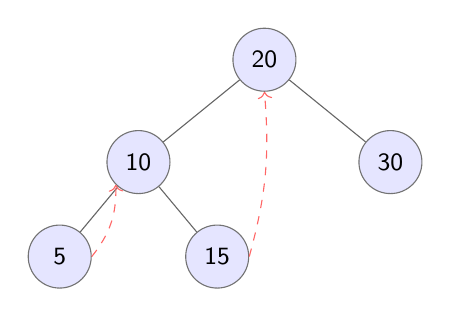
\begin{tikzpicture}[
  font=\sffamily\small,
  every node/.style={circle, draw=black!55, line width=0.4pt, minimum size=8mm, fill=blue!10, inner sep=0pt},
  edge/.style={draw=black!60, line width=0.4pt},
  thr/.style={->, dashed, draw=red!60, line width=0.4pt}
]
\node (n20) at (0, 2.5)    {20};
\node (n10) at (-1.6, 1.2) {10};
\node (n30) at (1.6, 1.2)  {30};
\node (n5)  at (-2.6, 0)   {5};
\node (n15) at (-0.6, 0)   {15};

\draw[edge] (n20) -- (n10);
\draw[edge] (n20) -- (n30);
\draw[edge] (n10) -- (n5);
\draw[edge] (n10) -- (n15);

\draw[thr] (n5.east)  to[bend right=20] (n10.south west);
\draw[thr] (n15.east) to[bend right=10] (n20.south);
\end{tikzpicture}
\end{document}
